% CS 111 style
% Typical usage (all UPPERCASE items are optional):
%       \input 111pre
%       \begin{document}
%       \MYTITLE{Title of document, e.g., Lab 1\\Due ...}
%       \MYHEADERS{short title}{other running head, e.g., due date}
%       \PURPOSE{Description of purpose}
%       \SUMMARY{Very short overview of assignment}
%       \DETAILS{Detailed description}
%         \SUBHEAD{if needed} ...
%         \SUBHEAD{if needed} ...
%          ...
%       \HANDIN{What to hand in and how}
%       \begin{checklist}
%       \item ...
%       \end{checklist}
% There is no need to include a "\documentstyle."
% However, there should be an "\end{document}."
%
%===========================================================
\documentclass[11pt,twoside,titlepage]{article}
%%NEED TO ADD epsf!!
\usepackage{threeparttop}
\usepackage{graphicx}
\usepackage{latexsym}
\usepackage{color}
\usepackage{listings}
\usepackage{fancyvrb}
%\usepackage{pgf,pgfarrows,pgfnodes,pgfautomata,pgfheaps,pgfshade}
\usepackage{tikz}
\usepackage[normalem]{ulem}
\tikzset{
    %Define standard arrow tip
%    >=stealth',
    %Define style for boxes
    oval/.style={
           rectangle,
           rounded corners,
           draw=black, very thick,
           text width=6.5em,
           minimum height=2em,
           text centered},
    % Define arrow style
    arr/.style={
           ->,
           thick,
           shorten <=2pt,
           shorten >=2pt,}
}
\usepackage[noend]{algorithmic}
\usepackage[noend]{algorithm}
\newcommand{\bfor}{{\bf for\ }}
\newcommand{\bthen}{{\bf then\ }}
\newcommand{\bwhile}{{\bf while\ }}
\newcommand{\btrue}{{\bf true\ }}
\newcommand{\bfalse}{{\bf false\ }}
\newcommand{\bto}{{\bf to\ }}
\newcommand{\bdo}{{\bf do\ }}
\newcommand{\bif}{{\bf if\ }}
\newcommand{\belse}{{\bf else\ }}
\newcommand{\band}{{\bf and\ }}
\newcommand{\breturn}{{\bf return\ }}
\newcommand{\mod}{{\rm mod}}
\renewcommand{\algorithmiccomment}[1]{$\rhd$ #1}
\newenvironment{checklist}{\par\noindent\hspace{-.25in}{\bf Checklist:}\renewcommand{\labelitemi}{$\Box$}%
\begin{itemize}}{\end{itemize}}
\pagestyle{threepartheadings}
\usepackage{url}
\usepackage{wrapfig}
\usepackage{hyperref}
%=========================
% One-inch margins everywhere
%=========================
\setlength{\topmargin}{0in}
\setlength{\textheight}{8.5in}
\setlength{\oddsidemargin}{0in}
\setlength{\evensidemargin}{0in}
\setlength{\textwidth}{6.5in}
%===============================
%===============================
% Macro for document title:
%===============================
\newcommand{\MYTITLE}[1]%
   {\begin{center}
     \begin{center}
     \bf
     CMPSC 300 and BIO 300 \\Introduction to Bioinformatics \\
     Fall 2017\\
     Oliver Bonham-Carter\\
     \url{http://www.cs.allegheny.edu/sites/obonhamcarter/cs300.html}
     \medskip
     \end{center}
     \bf
     #1
     \end{center}
}
%================================
% Macro for headings:
%================================
\newcommand{\MYHEADERS}[2]%
   {\lhead{#1}
    \rhead{#2}
    \immediate\write16{}
    \immediate\write16{DATE OF HANDOUT?}
    \read16 to \dateofhandout
    \lfoot{\sc Handed out on \dateofhandout}
    \immediate\write16{}
    \immediate\write16{HANDOUT NUMBER?}
    \read16 to\handoutnum
    \rfoot{Handout \handoutnum}
   }

%================================
% Macro for bold italic:
%================================
\newcommand{\bit}[1]{{\textit{\textbf{#1}}}}

%=========================
% Non-zero paragraph skips.
%=========================
\setlength{\parskip}{1ex}

%=========================
% Create various environments:
%=========================
\newcommand{\PURPOSE}{\par\noindent\hspace{-.25in}{\bf Purpose:\ }}
\newcommand{\SUMMARY}{\par\noindent\hspace{-.25in}{\bf Summary:\ }}
\newcommand{\DETAILS}{\par\noindent\hspace{-.25in}{\bf Details:\ }}
\newcommand{\HANDIN}{\par\noindent\hspace{-.25in}{\bf Hand in:\ }}
\newcommand{\SUBHEAD}[1]{\bigskip\par\noindent\hspace{-.1in}{\sc #1}\\}
%\newenvironment{CHECKLIST}{\begin{itemize}}{\end{itemize}}


\long\def\omitit #1{}

\begin{document}
\MYTITLE{Lab 7: Investigating Potential Virulence Factors in E. coli \\ 
\color{red}Save this lab assignment to: {\tt labs/lab7}\color{black}}
\MYHEADERS{Introduction to Bioinformatics}{Due: 1 Nov (2 weeks).}{Handed out on: 18 Oct. 2017}

\vspace*{-.1in}
\subsection*{Objectives}
\vspace*{-.1in}

\begin{itemize}
	\item Understand the use of a substitution matrix to score amino acid similarity in a protein sequence alignment.
	\item Gain experience using protein alignment to develop hypotheses about protein function based on sequence similarity.  
	\item Know how protein alignment differs algorithmically from DNA alignment.
	\item Know how substitution matrix is developed and how different matrices might be used to produce better alignments in particular situations.

\end{itemize}

\vspace*{-.1in}
\subsection*{Reading Assignment}
\vspace*{-.1in}
Chapter 5 in Exploring Bioinformatics textbook.

\vspace*{-.1in}
\subsection*{Part 1: Deliverable}
\vspace*{-.1in} 

Choose two candidate virulence factors from table on page 3.  For each factor you’ve selected, write a one-page summary discussing the factor’s likely function based on conserved domains and orthologous proteins.  Each summary should include a table with the organisms you’ve identified as having similar proteins, the known functions of those proteins, the quality of your BLAST matches, and the type of BLAST and substitution matrix used to generate the alignment.  Based on the evidence accumulated, is it reasonable to identify your protein as a virulence factor?  How would the function you have hypothesized for the protein contribute to the ability of EDL933 to cause disease?  Comment on the strength of your evidence:  How confident are you in assigning this function to your protein or in characterizing its role in virulence?  Be sure to include other tools and resources used in your characterization.


\vspace*{-.1in}
\subsection*{Part 1: Background}
\vspace*{-.1in} 

Escherichia coli (E. coli) is a very well known species of bacteria due to it being a major contributor to cases of food poisoning.  However, most strains of E. coli are harmless, or even beneficial, and reside in the large intestines of humans and other mammals.  One strain in particular, named O157:H7 is a highly virulent pathogen known to cause serious or even potentially fatal disease if as few as 10 cells are ingested.  What makes strain O157:H7 so different?

One key factor is O157:H7's acquisition of the gene for a toxin called Shiga toxin (Stx) not present in other E. coli strains.  Stx binds receptors found in human kidney tissue but, importantly, is not found in cattle, enabling these animals to be symptom-free carriers of the bacteria.  Genome sequencing has revealed many other differences between the O157:H7 genome and the genomes of ``tame'' E. coli inhabiting the human gut.  At least some of these genes specific to O157:H7 are likely to encode virulence factors: proteins such as Stx that contribute to the ability of the organism to cause disease.

Identifying and studying novel virulence genes evolved in or acquired by highly pathogenic strains of E. coli such as O157:H7 could be crucial for dealing with this important foodborne disease.  Understanding how these bacteria cause disease and why they have more severe effects than typical E. coli strains may lead us to new and better ways to treat and prevent disease.  

One of the first completely sequenced genomes was that of E. coli strain K-12 substrain MG1655.  This strain is a descendent of benign intestinal E. coli isolates.  Subsequently, a number of different E. coli genomes have been sequenced, including O157:H7 strains.  The first O157:H7 genome sequenced came from strain EDL933, isolated from contaminated ground beef from a McDonald's restaurant in Michigan.  Once genomes were sequenced, a key question was to find out how they differed.  

The degree of difference between the genomes of MG1655 and EDL933 is surprising:  MG1655 has more than 500,000 bases of sequence not found in EDL933, whereas more than 1.3 million bases of sequence unique to EDL933 were identified, including about one-forth of its 5,416 total genes.  Thus, hundreds of distinct genes could be virulence factors for EDL933.

Bioinformatics allows us to develop hypotheses about the functions of proteins.  Simply being present in in EDL933 but not MG1655 suggests that a gene could be a virulence factor.  Evidence to strengthen this hypothesis can be acquired by using protein alignment to look for orthologs of putative virulence proteins that have been identified and studied in other organisms.  Sequence similarity to a protein with a known virulence function or identification of protein domains suggestive of a virulence function are examples of such evidence.  

Much is known about bacterial virulence, and based on that background knowledge, we would expect virulence factors to function in roles such as toxins, systems for delivering toxins to host cells, components of pili and other bacterial surface features allowing attachment to host cells, enzymes that break down host proteins, and proteins that sequester iron and other nutrients.  However, it is important to bear in mind that even strong bioinformatics-based hypotheses require experimental testing - even minor sequence variations might result in altered functions or characterization of a gene with no obvious disease function might lead to the discovery of a new type of virulence factor.

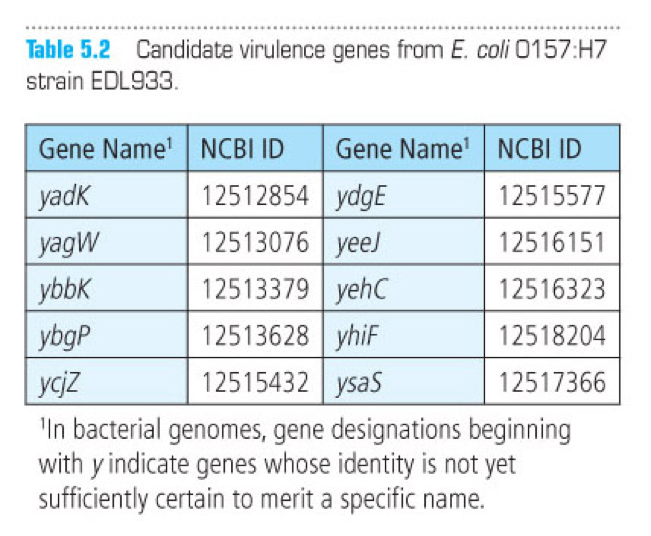
\includegraphics[scale=1]{table}


\vspace*{-.1in}
\subsection*{Part I Activity:  Using Protein Alignment to Explore Protein Function}
\vspace*{-.1in} 
BLAST – use BLAST to compare your protein sequence to known proteins in the NCBI database.  A protein BLAST incorporates a substitution matrix to score amino acid similarity.  

\begin{enumerate}
	\item Choose a potential virulence factor to invest age from the table.  Obtain the amino acid sequence in FASTA format using the NCBI protein database.

	\item From the BLAST home page, choose protein blast to align an amino acid sequence query with database sequences.  Paste the FASTA-formatted sequence into the BLAST query sequence box.

	\item  Use the Organism field to limit your search appropriately.  For example, you could choose to limit the search to Gram-negative bacteria or even the Enterobacteria (the large family of intestinal bacteria to which E. coli belongs).

	\item Add an additional Organisms field and use it to exclude E. coli from the search results – this prevents your results from being cluttered with high-scoring matches from EDL933 itself or other pathogenic E. coli strains.
	
	\item  At the bottom of the window, click Algorithm parameters to choose an appropriate substitution matrix: BLOSUM 62 is the default, but because the search is limited to relatively closely related organisms, perhaps it makes sense to try a matrix optimized for more closely related sequences such as BLOSUM 80 or PAM 70 (remember higher BLOSUM numbers and lower PAM numbers represent more similar sequences used to generate the matrix).

	\item Run your BLAST search. \\

Now comes the important work of analyzing the results.  Obviously, a high -scoring match (indicating a high degree of similarity between your query and some other protein) provides stronger evidence for a conserved function than a low-scoring match.  Similarly, a good alignment along the whole length of the protein better supports functional conservation than a partial match.  Review Chapter 4 of your textbook if necessary to refresh your memory of what the score and e-value mean.  

	\item  If you find a good match, investigate the function of the putative ortholog: Is it found in a pathogenic bacterium?  What is known about its function?  Is there evidence that it is a virulence factor?  Add this information to your one-page summary.
	
Conserved domains – a domain is a functional region of a protein.  For example, an energy-requiring enzyme might have an ATP-binding domain as well as a substrate-binding domain where its catalytic function is carried out.  A transcription factor would likely have a DNA-binding domain as well as a domain that interacts with RNA polymerase.  Even if two proteins are not terribly similar overall, they might have a particular domain in common:  Two DNA-binding proteins that have different functions might have similarity in their DNA-binding domains but be very different in a domain used for interactions with their distinct molecular partners.

While your BLAST search was running, you might have seen a page informing you that ``conserved domains'' have been detected in your query protein.  If so, you should see a box at the top of your BLAST results page titled Putative conserved domains have been detected.  BLAST looks for patterns in the query protein that resemble known functional domains and reports these results.  The conserved domain box shows the regions of your protein that are similar to well-characterized functional domains; clicking on this display takes you to more information about the conserved domains and the other proteins that contain them.  You can also run a conserved domain search directly without a BLAST search by searching NCBI’S Conserved Domains database.

	\item Were any conserved domains been detected in your query protein?  If so, investigate these domains and add this information to your one-page summary.
	
Substitution Matrices - What would happen if you changed the substitution matrix used in your search?  You initially optimized it to give higher scores to substitutions likely to occur in closely related sequences, but what if you used a matrix like PAM 250 or BLOSUM 45 that is based on more distantly elated sequences?  Although it is likely that the BLAST will still pick up the same high-scoring matches, there could be some less closely related proteins in the list, or you may notice changes in the score or e-value resulting from scoring mismatches.  

	\item  Change the substitution matrix and rerun your BLAST search.  Repeat for at least three different substitution matrices and inspect the results.  Note any interesting alignments in your one page summary.
	
What would happen if you searched for matches to really distantly related organisms?  Because the goal of this exercise is to identify potential virulence factors in E. coli it is appropriate to limit the matches to related bacteria, but perhaps you are curious to know whether your gene might have a human ortholog. Some bacteria-specific proteins have no identifiable human orthologs, whereas others have been conserved across this long span of evolutionary time.  Still others are surprisingly similar to human proteins, leading to speculation about recent horizontal transfer between species.  

	\item Use BLAST to determine if your gene has a human ortholog with a substitution matrix chosen to score such distant relationships appropriately.  Describe your findings in your one-page summary.

\end{enumerate}

\vspace*{-.1in}
\subsection*{Part 2: More Tools for Exploring Protein Function}
\vspace*{-.1in} 

Depending on your results for Part I, you may or may not have a strong, well-supported hypothesis regarding the function of your chosen genes.  Below are brief descriptions of additional tools that you may use to further investigate your genes.\\

\emph{PSI-BLAST}: PSI-BLAST is a variation of BLAST in which initial matches are used to refine the substitution matrix to identify even more distant matches.  This is a good tool when you want to identify meaning alignments to distantly related proteins, such as when a simple BLAST search reveals no good orthologs.  To use PSI-BLAST, start at the BLAST home page and choose protein BLAST as before, and then on the next page click on the PSI-BLAST button before start the search.\\

\emph{Pfam}: Pfam is a database of protein families – groups of proteins already shown to be similar in structure and function.  Particularly when a protein sequence of interest does not have a strong ortholog identifiable by a BLAST search or when the closest matches are partial or relatively low scoring, aligning the sequences with Pfam protein families may yield information about specific domains or regions of the protein.  When matches are found, the Pfam database provides considerable information about the known functions, sequences, and structures of the matching families, including links to still more information. \\

\emph{MOTIF}: Like Pfam, MOTIF looks for alignments between query amino acid sequence and functional domains and motifs (short sequence segments associated with some function).  The difference here is that MOTIF is a “meta site” that allows you to search up to six databases at once. \\

\emph{DAS}: The localization of a protein within a cell can also provide clues to possible functions.  DAS (dense alignment surface) deals with one aspect of protein localization: whether the protein contains potential transmembrane domains that would suggest it is an integral membrane protein.  Although there are various ways to approach this question (e.g. mapping hydrophobic amino acids), DAS uses an alignment-based approach in which it essentially looks for meaningful local alignments between the query protein and a set of unrelated known membrane proteins. \\

11.  Try some or all of the tools mentioned above to further your understanding of your potential virulence factor genes.  Add any new information you gain to your summary.  Don't forget to include which tools were used to find information and draw conclusions!

\omitit{
\vspace*{-.1in}
\subsection*{Part 3: BLAST through BioPython}
\vspace*{-.1in} 
Now, that you have investigated two candidate virulence factors in depth, you will perform a more extensive search using BioPython. 

For all candidate virulence factors from the table presented at the beginning of this document:

\begin{enumerate}
	\item Use BioPython do an Entrez search for each candidate. Save sequence into a separate output file using SeqIO module. Keep in mind, we are interested in proteins, not nucleotides, so you will need to make certain modifications.
	\item For each candidate, run your chosen protein sequence through BLAST using BioPython. Note, you must run your BLAST results using Python for this portion of the lab.  \\
	
Use four different matrices for each BLAST run of each candidate. Compare different matrices and discuss trends. You may gather and analyze some statistics, such as frequency, e-value, score information, etc. to perform your analysis. Report those results in a table similar to the one shown below, include your analysis summary and a table in your report.
\end{enumerate}

\begin{tabular}{|l|l|l|}
\hline
Gene Name & Stat1 & Stat2 \\
yadK & .. & .. \\
yagW & .. & .. \\
ybbK & .. & .. \\
ybgP & .. & .. \\
ycjZ & .. & .. \\
ydgE & .. & .. \\
yeeJ & .. & .. \\
yehC & .. & .. \\
yhiF & .. & .. \\
ysaS & .. & .. \\
\hline
\end{tabular}
}

\vspace*{-.1in}
\subsection*{Required Deliverables}
\vspace*{-.1in}
All of the deliverables specified below should be placed into a new folder named `lab06' in your Bitbucket repository ({\tt cs300f2017-bbill})  and shared with the instructor by correctly using  appropriate Git commands, such as {\tt git add -a}, {\tt git commit -m ``your message''} and {\tt git push} to send your documents to the Bitbucket's server. When you have finished, please ensure that you have sent your files correctly to the Bitbucket Web site by checking the {\tt source} files. This will show you your recently pushed files on their web site. Please ask questions, if necessary.
\color{red}
\begin{enumerate}
	\item A report addressing Parts 1 and 2.
	\item Make sure to submit a LibreOffice file, not a text file, with proper formatting and \textbf{your name included at the top of the document}.
\end{enumerate}
\color{black}

\noindent You should see the instructor if you have questions about assignment submission.
\end{document}



%%%%%%%%%%%%%%%
